\subsubsection{Termination}

When describing the shutdown of the whole system, we assumed the application
terminates gracefully.
In this section we show the algorithm we designed to achieve this goal.

As we can see from figure \ref{fig:termination-app}, the termination follows the
opposite order of the bootstrap.

\begin{figure}[H]
  \centering
  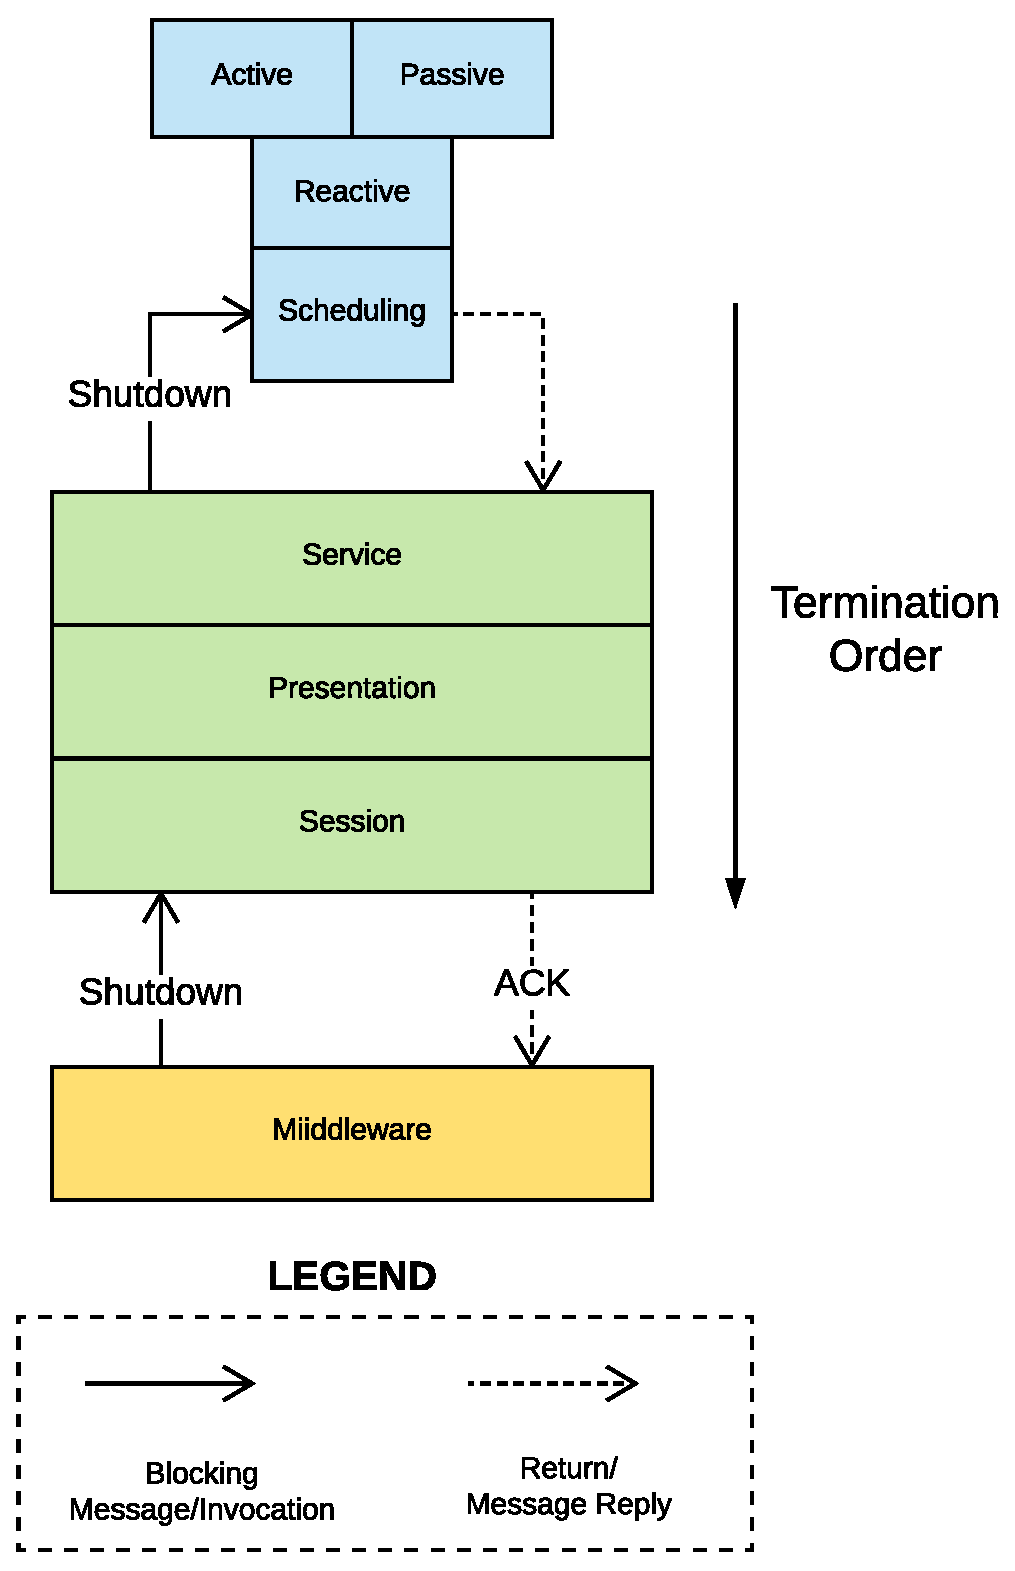
\includegraphics[scale=0.4,keepaspectratio]
    {images/solution/termination-app.eps}
  \caption{Application Termination}
  \label{fig:termination-app}
\end{figure}

%TODO: Review termination process
\begin{enumerate}
  \item The middleware sends a \verb|shutdown| message to IL;
  \item The upwards components\footnote{these components carry the messages
  from middleware to the application layer} of the sublayers of IL terminates
  themselves when they
  read the shutdown request in the header. This is achieved by a transition
  from \verb|active| to \verb|stopped| state, which enables the master
  of each event loop to wait for all its workers to complete. Then the master
  puts the shutdown notification in the queue of the next IL component;
  \item The shutdown message is forwarded upwards until it reaches the Scheduling
  component. Then the scheduler notifies its workers. The workers change their
  state to \verb|stopped| and wait on a barrier until all the other workers have
  completed their execution. \\
  At this stage, we have the guarantee that no worker is running at
  the Application Layer level. Indeed, all the Application Layer
  entities are inerts because their engine (i.e., the scheduler) has been
  turned off;
  \item The previous point implies that we can safely terminate
  also the downwards components of the IL subsytem. Indeed, no message
  will be sent if the scheduler is not running. Thus, as last message
  an acknowledgment to the shutdown request
  originally sent by the middleware is packed
  by the stub component and sent downwards through the IL forwarding pipeline;
  \item All the downwards components of IL behaves exactly as the upwards one;
  \item The sender component forwards the acknowledgment message
  to the middleware.
\end{enumerate}


We implement also a dump method, to enable each stateful entity to save its
state before terminating. However we have not
been able to test it successfully in the distributed environment. Thus, we
kept it in the source code but we did not use it in production.



Similarly to the bootstrap phase, the middleware expects to receive the
\verb|shutdown| ack message within a certain amount of time.
In order to do so, when sending the message, the middleware starts a timeout.
Wherefore if it expires before receiving a response message,
it retransmit again the \verb|shutdown| request towards the application.
